\documentclass[12pt, letterpaper]{article}
\usepackage[utf8]{inputenc}
\usepackage[T2A]{fontenc}
\usepackage[english, russian]{babel} % выравнивание 
\usepackage[a4paper,% размер страницы
text={180mm, 260mm},% ширина и высота текста
top=15mm, bottom=15mm, left=15mm, top=15mm]{geometry}
\usepackage{textcomp}
\usepackage{graphicx}


\graphicspath{ {../img} }

\title{SmartCalc v1.0}
\author{Almetate}
\date{February 2023}

\begin{document}
\maketitle

Программа разработана на языке Си стандарта C11 с использованием компилятора gcc.

Исходный код программы находится в папке src.
Сборка программы настроенна с помощью MakeFile со стандартным набором целей для GNU-программ. Установка идет в папку build.

Обеспечено покрытие unit-тестами модулей, связанных с вычислением выражений, с помощью библиотеки Check
Реализован графический пользовательский интерфейс на базе фреймворка Qt-5.

На вход программы могут подаваться как целые числа, так и вещественные числа, записанные через точку. Вычисление производиться после полного ввода вычисляемого выражения и нажатия на символ `=`.

Вычисление произвольных скобочных арифметических выражений в инфиксной нотации.
Вычисление произвольных скобочных арифметических выражений в инфиксной нотации с подстановкой значения переменной x в виде числа.

Алгоритм работы SmartCalc основан на способе Обратной польской нотации с использованием стэка.

Область определения и область значения функций ограничиваются числами от -1000000 до 1000000.
Для построения графиков функции необходимо дополнительно указывать отображаемые область определения и область значения.

Для корректной проверки и работы над данным проектом необходимо:

-Qt Creator 6.0.2 или выше - для графического интерфейса

-LaTeX - для компиляции документации

Внешний вид калькулятора:
  
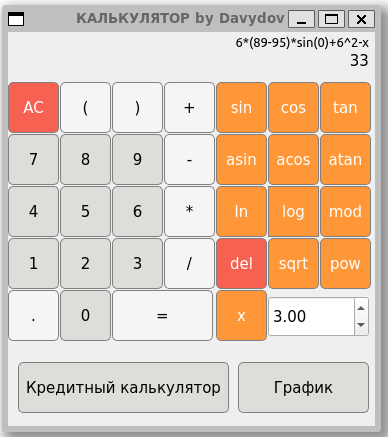
\includegraphics[scale=0.65]{calc.eps}

Пример получаемого графика:

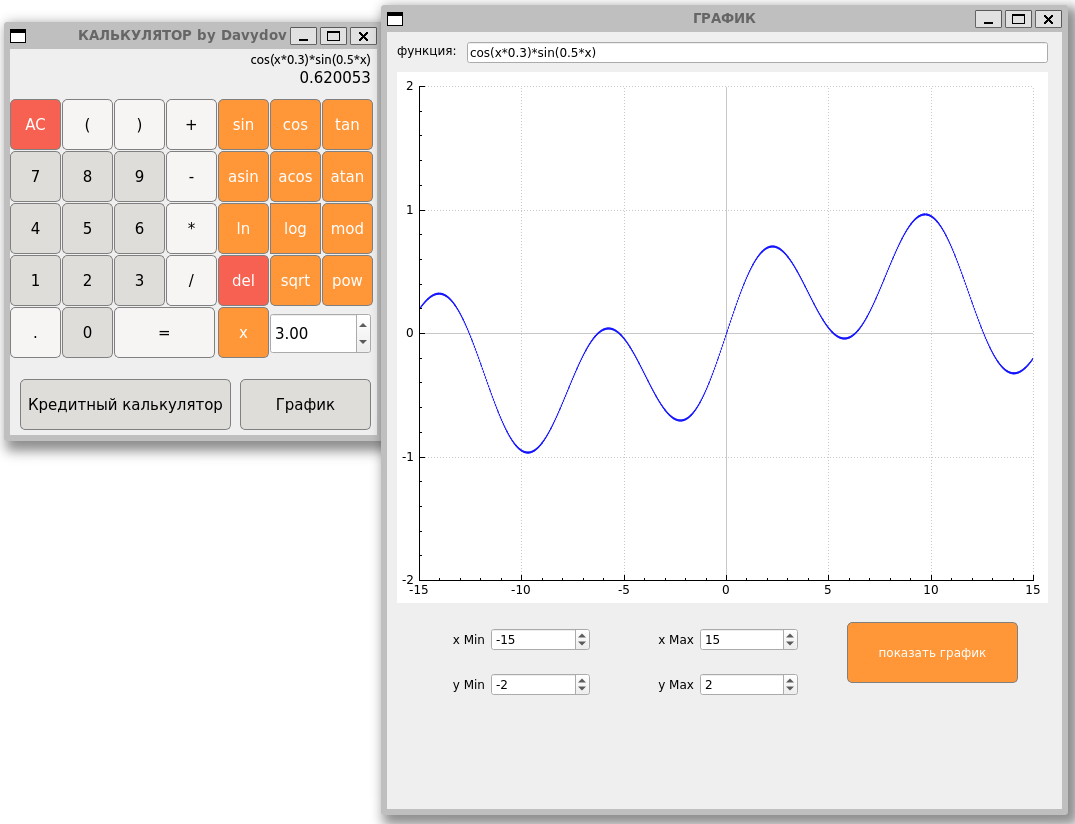
\includegraphics[scale=0.5]{graph.eps}

Пример расчета ежемесячных платежей с использованием кредитного калькулятора

\includegraphics[scale=0.45]{credit_calc.eps}

\end{document}